\vspace{1cm}{\bf Calibration [Omar]}


Description of hit amplitude, baseline/gain calibration, noisy channels/chips, pulse shape cuts, occupancy. 

Plots: Response plot, gain, noisy channels vs run nr?, data/MC of noise hits,Data/MC plot of occupancy for some layers  

\vspace{1cm}{\bf Cluster reconstruction [Omar]}


Description of the cluster reconstruction.

Plots: mip distribution

\vspace{1cm}{\bf SVT timing [Sho]}

The time reconstruction algorithm described in \ref{sec:svtŧ} was used to fit a single hit to each SVT channel in each event.
Pileup was not considered due to the very low hit rate in the SVT.

As shown in Figure \ref{fig:apvfit}, values of fit $\chi^2$ fell in the distribution of $\chi^2$ for 4 degrees of freedom (6 points -- 2 fit parameters).

\begin{figure}[ht]
	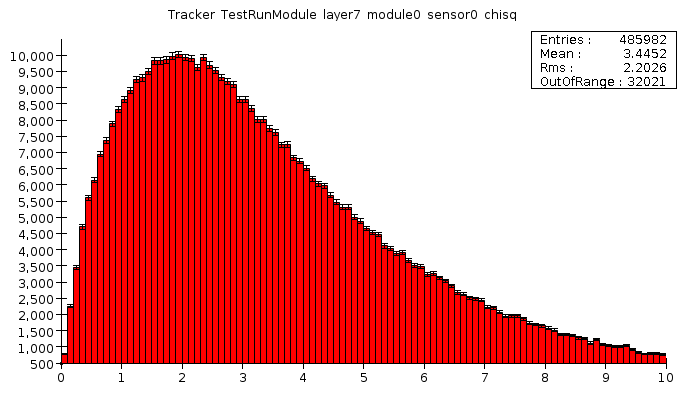
\includegraphics[width=\textwidth]{test2012/svtperformance/apvfit_chisq}
	\caption{\small{Histogram of $\chi^2$ values for pulse fits for all channels on a representative sensor. Peak at 2 is consistent with dof of 4, as expected.} }
	\label{fig:apvfit}
\end{figure}

After clustering these hits, the hit time for the cluster is computed as the amplitude-weighted average of the channel hit times. 



Since we have no measurement of the ``true'' hit time, we use the average of all cluster times in a track as the ``track time,'' and take the residual of the cluster time relative to that.
The track time, shown in Figure \ref{fig:tracktime}, has the expected amount of trigger jitter.
Different sensors have systematic offsets in hit time (up to a couple ns) due to time of flight and variations between readout chips. 
We correct these offsets so that the time residual is centered around 0 for each sensor. The RMS of the residual (from a Gaussian fit to the residual histogram, Figure \ref{fig:timeres}) is roughly 2.4 ns for each sensor.

\begin{figure}[ht]
	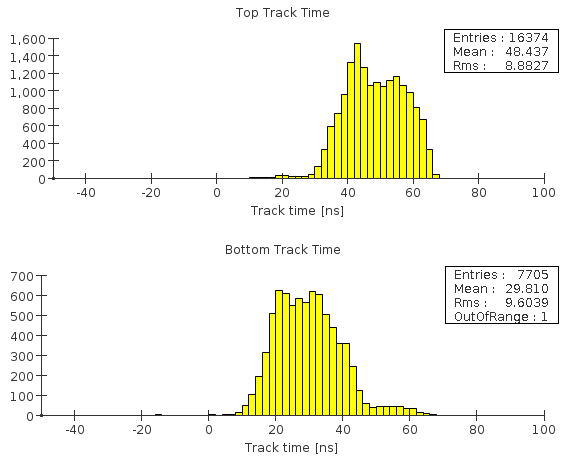
\includegraphics[width=\textwidth]{test2012/svtperformance/track_time}
	\caption{\small{Track time distribution, measured relative
	to the APV25 clock, for top and bottom tracks. The
width of the distribution is due to trigger jitter (24 ns
jitter in tracker readout clock, plus 16 ns jitter in the
trigger system). The shift between top and bottom
is due to a trigger time shift between the two halves
of the ECal.} }
	\label{fig:tracktime}
\end{figure}


Because the track time is calculated using the individual hit times, the hit time is positively correlated with the track time; thus the RMS of the residual is slightly smaller than the true time resolution.
The standard deviation of this residual for $n$-hit tracks where all hits have the same time resolution is reduced by a factor of $\sqrt{(n-1)/n}$; since most of our tracks have 8 clusters, the true time resolution is 2.6 ns. 

\begin{figure}[ht]
	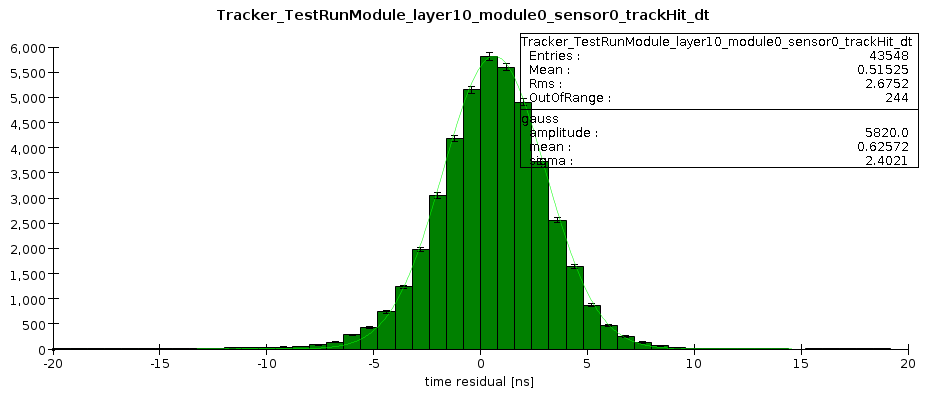
\includegraphics[width=\textwidth]{test2012/svtperformance/timeres}
	\caption{\small{Histogram and Gaussian fit of residual of cluster times for a representative sensor, relative to the track time. Because the cluster times and track time have positive covariance, the true time resolution is slightly larger than the standard deviation shown here.} }
	\label{fig:timeres}
\end{figure}

%\begin{figure}[ht]
%	\includegraphics[width=\textwidth]{test2012/svtperformance/hit_dt}
%	\caption{\small{} }
%	\label{fig:hit_dt}
%\end{figure}

This is somewhat worse than the $\approx 2$ ns resolution expected, but we believe this discrepancy is due to our fit function. Our pulse shape fit assumes an ideal CR-RC pulse shape; since the actual pulse shape has a slower rise time, there is a systematic pull on the hit time when a hit comes immediately before the APV clock time. 
This is visible in Figure \ref{fig:timeres_2D} as a shift in the residual at certain values of track time.
Work is in progress to use the actual pulse shape in time reconstruction; this should improve time resolution.

\begin{figure}[ht]
	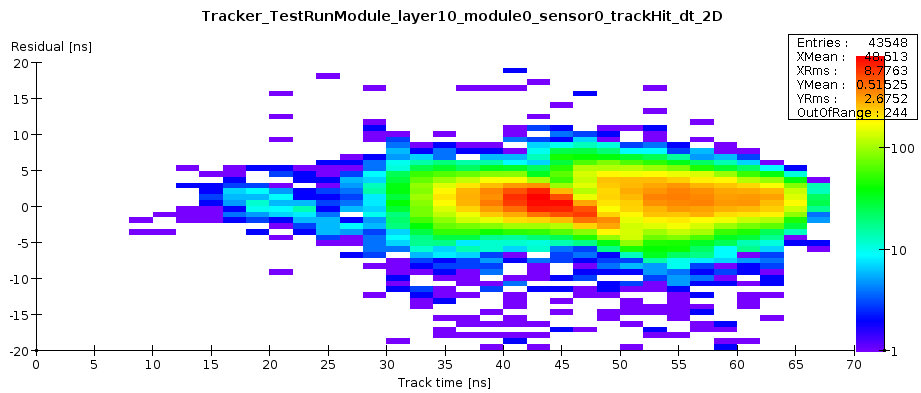
\includegraphics[width=\textwidth]{test2012/svtperformance/timeres_2D}
	\caption{\small{Plot of the time residual for a representative sensor vs. the track time. 
		The kinks in the horizontal band are caused by the fitter; without them the 1-D histogram in Figure \ref{fig:timeres} (the projection of this histogram) would be narrower.} }
	\label{fig:timeres_2D}
\end{figure}

\vspace{1cm}{\bf Tracking algorithms [Matt/Omar]}


Pattern recognition/Stereo hit reconstruction and description of the tracking algorithm. 

Plots: tracking efficiency vs run nr, hit efficiency vs run nr for data. Overlay MC.

\vspace{1cm}{\bf Tracking algorithms [Matt]}


Analysis of two track events. 

Plots: invariant mass, vertex position, 2-track event multiplicity. Compare with MC for all these 
